\begin{figure*}[t]
\centering
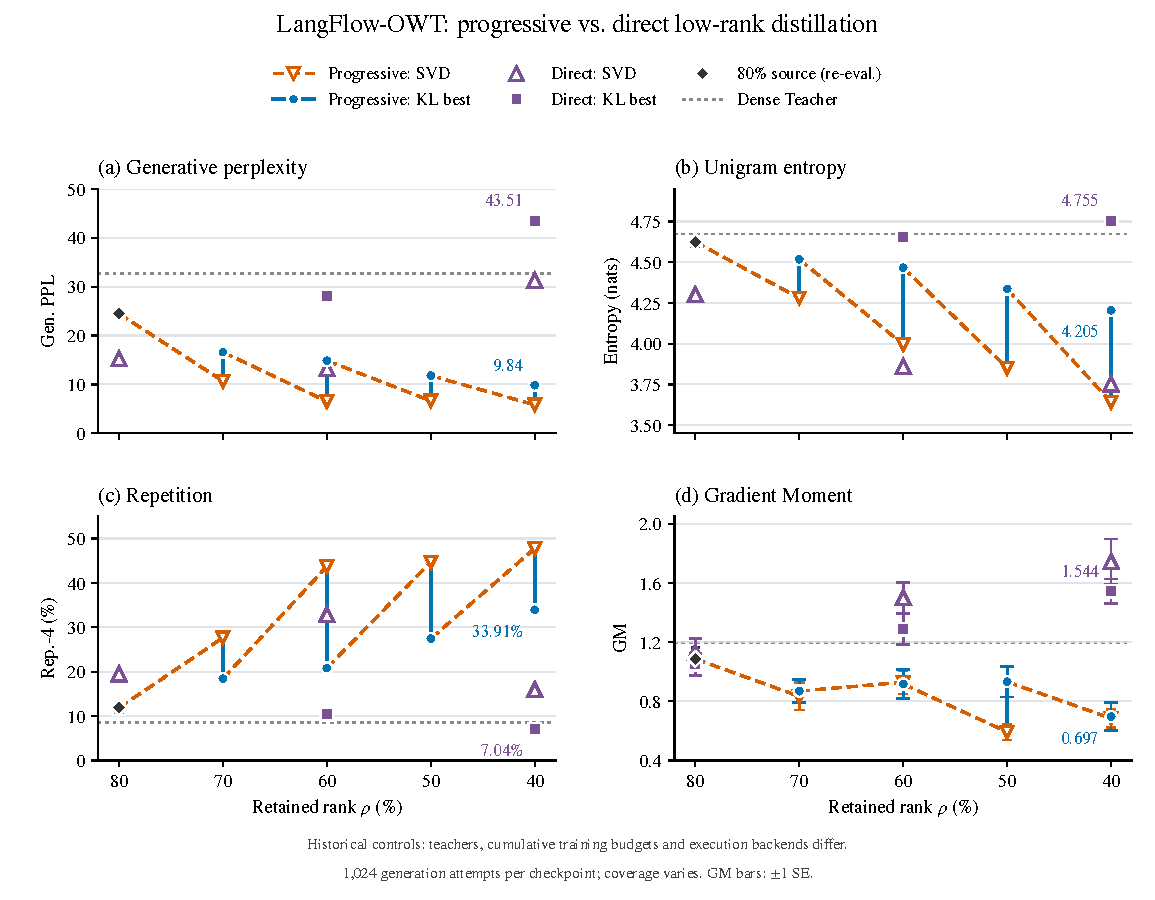
\includegraphics[width=\textwidth]{progressive_vs_direct.pdf}
\caption{Progressive versus independent low-rank distillation on LangFlow-OWT.
Orange dashed segments show truncation from the preceding best student; blue
vertical segments show subsequent KL distillation. Purple open triangles and
filled squares show independent SVD from the dense Teacher and distillation
against that Teacher. Independent points are measured only at 80\%, 60\%, and
40\%. Gray dotted lines denote the dense Teacher. The black 80\% source and
purple 80\% KL marker are separate evaluations of the same checkpoint.
The scoring protocol and GM reference texts are shared. This historical
comparison differs in teacher targets, stage caps (5,000 updates for direct;
10,000 for progressive), cumulative training exposure, and generation backends
(eager versus compiled). Each checkpoint attempts 1,024 samples. The direct
40\% SVD point uses 980 scorable texts and 469 GM pairs; other displayed points
use 1,014--1,024 texts and 502--512 pairs. GM bars denote $\pm$ one standard error.}
\label{fig:progressive_vs_direct}
\end{figure*}
